\documentclass{article}
\AtBeginDocument{\RenewCommandCopy\qty\SI}
\usepackage{style}
\title{ECE355 Cheatsheet}
\author{Hanhee Lee}
\lhead{ECE355}
\rhead{Hanhee Lee}

\begin{document}
\maketitle

\tableofcontents

\listoffigures

\listoftables

\section{Tips}
\begin{intuition}
    \begin{itemize}
        \item May diverge from textbook, but only responsible for lecture content.
        \item Tutorials: Review of last week's topics and assigned problems. 
        \item Piazza for asking questions.
        \item ISM: Investigate topic of interest that uses signals or systems with 10 pages that are reference, explain concepts in your own way.
        \item Quiz every week except for term tests. 
        \item 30 minutes, appears Tuesday morning and ends Tuesday night. 
        \item Easier than usual questions that tests understanding. 
        \item Open book with MC, numerical answer. 
    \end{itemize}
\end{intuition}

\section{Mathematical Review}
\subsection{Sets}
\begin{definition}
    An unordered collection of objects (i.e. elements or members)
    \begin{itemize}
        \item A set \emph{contains} its elements or elements of a set are \emph{contained in} that set.
    \end{itemize}
\end{definition}

    \subsubsection{Set notation}
    \begin{terminology}
        \begin{itemize}
            \item $\ldots$ mean "and so on"
            \item $:$ mean "such that"
            \item $\in$ mean "contained"
            \item $\notin$ mean "not contained"
            \item $\emptyset$ mean "empty set (i.e. a set contains no elements")
            \item $A\subseteq B$ mean "Only if every element of $A$ is also an element of $B$"
            \item $B\supseteq A$ mean "B is a superset of A to mean A is a subset of B" 
            \item Normally, elements of a set are listed just once.
        \end{itemize}
    \end{terminology}

\begin{example}

    \textbf{Sets:}
    \begin{itemize}
        \item $E = \{0,2,4,6,8\}$, where $2\in E$ and $1 \notin E$
        \item $\mathbb{Z} = \{\ldots,-2,-1,0,1,2,\ldots\}$
        \item $P=\{0,1,...,255\}$
        \item $O = \{x \in \mathbb{Z}: \; x=2k+1 \text{ for some } k \in \mathbb{Z}\}$
        \item $\{\emptyset,\{\emptyset\}\}$ (i.e. A set that has other sets as elements).
    \end{itemize}
    \vspace{1em}

    \textbf{Subset:}
    \begin{itemize}
        \item $E \subseteq \mathbb{Z}$
    \end{itemize}
\end{example}

\begin{theorem}
    $A = B$ means $A \subseteq B$ and $B \subseteq A$.
    \begin{itemize}
        \item \textbf{Note:} Have to prove in both directions.
    \end{itemize}
\end{theorem}

\begin{example}
    $\{1,2,3\}=\{3,2,1,1,2\}$
\end{example}

    \subsubsection{Important sets}
    \begin{definition}
        \begin{enumerate}
            \item \textbf{Natural:} \( \mathbb{N} = \{0, 1, 2, 3, \dots \} \): 
            \item \textbf{Integers:} \( \mathbb{Z} = \{ \dots, -2, -1, 0, 1, 2, \dots \} \): 
            \item \textbf{Rational:} \( \mathbb{Q} = \left\{ \frac{a}{b} : a, b \in \mathbb{Z}, b \neq 0 \right\} \): 
            \item \textbf{Real:} \( \mathbb{R} \): 
            \item \textbf{Complex:} \( \mathbb{C} = \{ a + bj : a, b \in \mathbb{R} \} \)
            \begin{itemize}
                \item \( j \): imaginary unit, where \( j^2 = -1 \) and \( j = \sqrt{-1} \)
            \end{itemize}
        \end{enumerate}  
        \begin{itemize}
            \item \textbf{Note:} $\mathbb{N} \subseteq \mathbb{Z} \subseteq \mathbb{Q} \subseteq \mathbb{R} \subseteq \mathbb{C} $
        \end{itemize}      
    \end{definition}

\subsection{Ordered n-tuples}
\begin{definition}
    An ordered collection of \( n \) elements, where \( n \) is a positive integer, denoted as \( (a_1, a_2, \dots, a_n) \), where \( a_1 \) is the first element, and so on, up to \( a_n \).
\end{definition}
    
    \subsubsection{How are two tuples equal?}
    \begin{definition}
        Unlike sets, both the order of elements and the repetition of values are significant. Therefore, two ordered \( n \)-tuples are considered equal (i.e. $(a_1, a_2, \dots, a_n) = (b_1, b_2, \dots, b_n)$) iff:

        \[
        a_1 = b_1, a_2 = b_2, \dots, a_n = b_n.
        \]
    \end{definition}

    \subsubsection{Cartesian product}
    \begin{definition}
        \textbf{Two sets:}
        The \textit{Cartesian product} of two sets \( A \) and \( B \) (in that order), denoted as \( A \times B \), is the set of all \textit{ordered pairs} or \textit{ordered 2-tuples} \( (a, b) \) where \( a \in A \) and \( b \in B \). Thus

        \begin{equation}
            A \times B = \{ (a, b) : a \in A, b \in B \}.    
        \end{equation}
        \begin{itemize}
            \item \textbf{General:} $B \times A \neq A \times B$
            \item \textbf{2-fold Cartesian product:} $A \times A$ is denoted as $A^2$
        \end{itemize}
        \vspace{1em}

        \textbf{More than two sets:}
        The Cartesian product of sets \( A_1, A_2, \dots, A_n \), denoted as \( A_1 \times A_2 \times \cdots \times A_n \), is the set of ordered \( n \)-tuples \( (a_1, a_2, \dots, a_n) \), where \( a_1 \in A_1, a_2 \in A_2, \dots, a_n \in A_n \). Thus

        \begin{equation}
            A_1 \times A_2 \times \cdots \times A_n = \{(a_1, a_2, \dots, a_n) : a_1 \in A_1, a_2 \in A_2, \dots, a_n \in A_n\}.
        \end{equation}
        \begin{itemize}
            \item \textbf{n-fold Cartesian product:} $A\times A\times \cdots \times A$ is denoted as $A^n$
        \end{itemize}

    \end{definition}

\subsection{Functions}
\begin{definition}
    A function \( f: A \to B \) from a set \( A \) (the domain of \( f \)) to a set \( B \) (the codomain of \( f \)) assigns to each element \( a \in A \) exactly one element \( b \in B \), usually denoted as \( b = f(a) \).
\end{definition}

    \subsubsection{Range/Image}
    \begin{definition}
        \textbf{The range or image} of \( f \) is the subset of the codomain $B$ given as 
        \[
        \text{Im}_f(A) = \{ b \in B: \exists a \in A(f(a) = b) \}.
        \]
        \begin{itemize}
            \item \textbf{English:} Set of values "hit" by $f$ as its argument ranges over the set $A$.
        \end{itemize}
    \end{definition}

    \subsubsection{Inverse Image}
    \begin{definition}
        \textbf{The inverse image or pre-image} of any element \( b \in B \) under the mapping by \( f \) is the set 
        \[
        f^{-1}(b) = \{ a \in A : f(a) = b \}.
        \]
        \begin{itemize}
            \item \textbf{English:} Set of elements of the domain that map to $b$ under transformation by $f$.
            \item \textbf{Key:} If $b$ is an element of the codomain that is not in the range of $f$, then $f^{-1} (b) = \emptyset$
        \end{itemize}
    \end{definition}

\begin{example}
    \begin{itemize}
        \item Domain of \( g \): \( A = \{ 1, 2, 3, 4 \} \)
        \item Codomain of \( g \): \( B = \{ w, x, y, z \} \)
        \item Image of \( A \): \( \text{Im}_g(A) = \{ w, x, z \} \subseteq B \)
        \item Inverse Image
        \[
        g^{-1}(w) = \{ 1 \}
        \]
        \[
        g^{-1}(x) = \{ 2, 4 \}
        \]
        \[
        g^{-1}(y) = \emptyset
        \]
        \[
        g^{-1}(z) = \{ 3 \}
        \]
    \end{itemize}
    
    % Mapping Diagram
    \begin{center}
    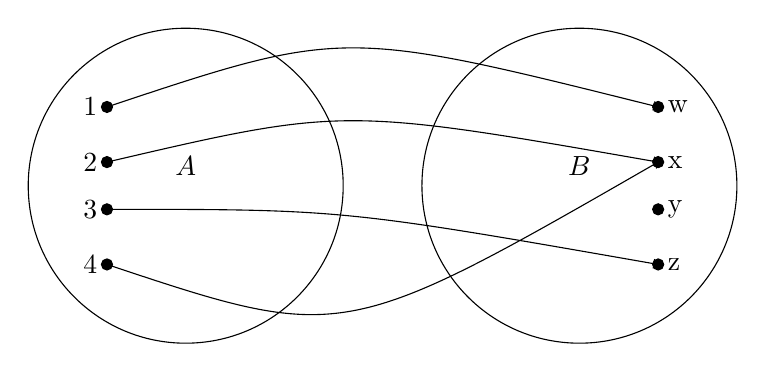
\begin{tikzpicture}
        % Sets A and B
        \draw (0, 0) circle (2cm) node[anchor=south] {$A$};
        \draw (5, 0) circle (2cm) node[anchor=south] {$B$};
    
        % Elements in A
        \filldraw[black] (-1, 1) circle (2pt) node[anchor=east] {1};
        \filldraw[black] (-1, 0.3) circle (2pt) node[anchor=east] {2};
        \filldraw[black] (-1, -0.3) circle (2pt) node[anchor=east] {3};
        \filldraw[black] (-1, -1) circle (2pt) node[anchor=east] {4};
    
        % Elements in B
        \filldraw[black] (6, 1) circle (2pt) node[anchor=west] {w};
        \filldraw[black] (6, 0.3) circle (2pt) node[anchor=west] {x};
        \filldraw[black] (6, -0.3) circle (2pt) node[anchor=west] {y};
        \filldraw[black] (6, -1) circle (2pt) node[anchor=west] {z};
    
        % Arrows for mappings
        \draw[->] (-1, 1) .. controls (2, 2) .. (6, 1);  % 1 -> w
        \draw[->] (-1, 0.3) .. controls (2, 1) .. (6, 0.3);  % 2 -> x
        \draw[->] (-1, -0.3) .. controls (2, -0.3) .. (6, -1);  % 3 -> z
        \draw[->] (-1, -1) .. controls (2, -2) .. (6, 0.3);  % 4 -> x
    \end{tikzpicture}
    \end{center}    
\end{example}

    \subsubsection{Injective}
    \begin{definition}
        A function \( f: A \to B \) is called injective (or an injection or one-to-one) if $\forall a_1 \forall a_2$
        \[
        a_1 \neq a_2 \rightarrow f(a_1) \neq f(a_2).
        \]
        \[
        (f(a_1) = f(a_2) \rightarrow a_1 = a_2)
        \]

        \begin{itemize}
            \item \textbf{English:} Maps distinct elemetns of the domain to distinct elements of the codomain.
        \end{itemize}
        \customFigure[0.25]{00_Images/Injective.png}{Injective function.}
    \end{definition}

    \begin{process}
        Show a function is injective:
        \begin{enumerate}
            \item Set $f(x_1) = f(x_2)$
            \item Prove $x_1 = x_2$ from step 1. 
        \end{enumerate}
        \vspace{1em}

        Show a function is not injective:
        \begin{enumerate}
            \item Find a counterexample where $f(a_1) = f(a_2)$.
        \end{enumerate}
    \end{process}

    \subsubsection{Surjective}
    \begin{definition}
        A function \( f: A \to B \) is called surjective (or a surjection or onto) if 
        \[
        \forall b (f^{-1}(b) \neq \emptyset), \quad \text{or} \quad \forall b \exists a (f(a) = b),
        \]
        \begin{itemize}
            \item \textbf{English:} Every element in the codomain has a mapping back to the domain.
        \end{itemize}

        \customFigure[0.25]{00_Images/Surjective.png}{Surjective function.}
    \end{definition}

    \begin{process}
        Show a function is surjective:
        \begin{enumerate}
            \item Find the inverse of $f(x)=y$ by writing $x$ in terms of $y$ denoted $f^{-1}$
            \item See if the inverse satisfies the codomain, and there is no empty set.
        \end{enumerate}
        \vspace{1em}

        Show a function is not surjective:
        \begin{enumerate}
            \item Find a counterexample, where you get the empty set for $b\in B$
        \end{enumerate}
    \end{process}

    \begin{warning}
        Any nonsurjective function is a surjective function obtained from the original function by having the codomain match the range.
    \end{warning}

    \subsubsection{Bijective}
    \begin{definition}
        A function \( f: A \to B \) that is both injective and surjective is called bijective (or a bijection or a one-to-one correspondence).
        \begin{itemize}
            \item \textbf{Correspondence:} Inverse exists
        \end{itemize}
        \customFigure[0.25]{00_Images/Bijective.png}{Bijective function.}
    \end{definition}

    \subsubsection{Composition of g with f}
    \begin{definition}
        If \( f: A \to B \) and \( g: B \to C \), then \( g \circ f: A \to C \) s.t. $a \rightarrow g(f(a))$ (i.e. first apply $f$, then apply $g$)
        
        \customFigure[0.5]{00_Images/Composition.png}{Composition example}
        \begin{itemize}
            \item \textbf{Order is important:} $ f(g(a)) \neq g(f(a)) $
        \end{itemize}
    \end{definition}

    \subsubsection{Identity map}
    \begin{definition}
        \[
        \text{id}_A: A \to A \quad \text{id}(a) = a \; \forall a \in A
        \]
    \end{definition}

    \subsubsection{Bijective property}
    \begin{definition}
        Let \( f: A \to B \), then iff \( f \text{ is bijective, } \exists \text{ a function } f^{-1}: B \to A \text{ s.t. } f^{-1} \circ f = \text{id}_A \text{ and } f \circ f^{-1} = \text{id}_B \).
        \customFigure[0.5]{00_Images/Bijective_Property.png}{Illustration of bijective function}
    \end{definition}

    \subsubsection{Set of all functions with domain and codomain}
    \begin{definition}
        The set of all fcns with domain $A$ and codomain $B$ is itself a set denoted $B^A$.
    \end{definition}

\begin{example}
    % Example of the set of all functions from A to B
    If \( A = \{1, 2\} \) and \( B = \{x, y, z\} \), then \( B^A \) has \( 3^2 = 9 \) elements (i.e., \( B^A \)).

    \[
    f = \left( \begin{array}{c c}
    1 & 2 \\
    f(1) & f(2) \\
    \end{array} \right)
    \]

    The set \( B^A \) is:

    \[
    B^A = \left\{
    \left( \begin{array}{c c}
    1 & 2 \\
    x & x \\
    \end{array} \right),
    \left( \begin{array}{c c}
    1 & 2 \\
    x & y \\
    \end{array} \right),
    \left( \begin{array}{c c}
    1 & 2 \\
    x & z \\
    \end{array} \right),
    \left( \begin{array}{c c}
    1 & 2 \\
    y & x \\
    \end{array} \right),
    \left( \begin{array}{c c}
    1 & 2 \\
    y & y \\
    \end{array} \right),
    \left( \begin{array}{c c}
    1 & 2 \\
    y & z \\
    \end{array} \right),
    \left( \begin{array}{c c}
    1 & 2 \\
    z & x \\
    \end{array} \right),
    \left( \begin{array}{c c}
    1 & 2 \\
    z & y \\
    \end{array} \right),
    \left( \begin{array}{c c}
    1 & 2 \\
    z & z \\
    \end{array} \right)
    \right\}
    \]
\end{example}

\subsection{Complex math}
    \subsubsection{Complex number basics}
    \begin{definition}
    \begin{itemize}
        \item \( z = a + bj \), where \( a, b \in \mathbb{R} \)
        \begin{itemize}
            \item \( \text{Re}(z) = a \)
            \item \( \text{Im}(z) = b \)
        \end{itemize}
        
        \item \textbf{Complex conjugate:} If \( z = a + bj \), then \( z^* = a - bj \).
        
        \item \textbf{Magnitude:} \( |z| = \sqrt{z \cdot z^*} = \sqrt{a^2 + b^2} \).
    \end{itemize}

        % Complex plane diagram
        \begin{center}
        \begin{tikzpicture}
            \draw[->] (-0.5, 0) -- (3, 0) node[anchor=north] {$Re$};
            \draw[->] (0, -0.5) -- (0, 3) node[anchor=east] {$Im$};
            \filldraw[black] (2, 2) circle (2pt) node[anchor=south west] {$(a, b)$};
            \draw[->] (0, 0) -- (2, 2);
            \node at (2.3, -0.3) {$a$};
            \node at (-0.3, 2.3) {$b$};
        \end{tikzpicture}
        \end{center}

    \end{definition}

    \begin{example} 
        Expand the following function:
        \begin{align*}
            (a + bj)(c + dj) &= ac + (bc + ad)j + bdj^2 \\
            &= ac + (bc + ad)j - bd \quad \text{since} \, j^2 = -1.
        \end{align*}
    \end{example}

    \subsubsection{Complex exponential function}
    \begin{definition}
        % Exponential function definition
        \begin{equation}
            \exp: \mathbb{C} \to \mathbb{C} \text{ via } \exp(z) = 1 + z + \frac{z^2}{2!} + \frac{z^3}{3!} + \cdots = \sum_{k=0}^{\infty} \frac{z^k}{k!}    
        \end{equation}
        \begin{itemize}
            \item \textbf{Entire function:} Convergent no matter the values of z.
        \end{itemize}
        
        Let \( \theta \in \mathbb{R} \), the expansion of \( \exp(j\theta) \) is:
        \begin{equation}
            \exp(j\theta) = \cos \theta + j \sin \theta 
        \end{equation}
    \end{definition}

    \subsubsection{Complex plane with radius r}
    \begin{intuition}
        \customFigure[0.5]{00_Images/Complex_Plane_General.png}{Complex plane in general with radius r.}

        \begin{itemize}
            \item \textbf{Bounds:} $r \geq 0$ and $-\pi < \theta \leq \pi$
            \item \textbf{Polar:} Multiplication
            \item \textbf{Rectangular:} Additive
        \end{itemize}
    \end{intuition}

    \subsubsection{Complex conjugate}
    \begin{definition}
        \begin{equation}
            z^* = re^{-j\theta}
        \end{equation}
    \end{definition}

    \subsubsection{Converting between polar and rectangular form}
    \begin{process}

        \textbf{Polar to rectangular:} $e^{j\theta}$
        \begin{enumerate}
            \item Find $r$ and $\theta$ from $re^{j\theta}$
            \item Write in rectangular form: $z=rcos\theta + jrsin\theta$
        \end{enumerate}

        \textbf{Rectangular to polar:} $a+bj$
        \begin{enumerate}
            \item Find $r$ using Pythagorean theorem: $r = \sqrt{a^2 + b^2}$
            \item Find $\theta$ using trigonometry: $\theta = \text{tan}^{-1} \left(\frac{b}{a}\right)$, where $b$ is the opposite and $a$ is adjacent.
            \item Write in polar form: $z=re^{j\theta}$
        \end{enumerate}
        \begin{itemize}
            \item \textbf{Note:} Both forms can be found intuitively through a drawing of the complex plane. 
        \end{itemize}
    \end{process}

\subsection{Propositional logic}
    \subsubsection{Proposition}
    \begin{definition}
        A declarative statement that can be either \emph{true} or \emph{false}, denoted by a symbol (e.g. p or q).
    \end{definition}

    \subsubsection{Compound proposition}
    \begin{definition}
        Formed from existing propositions via negation and logical connectives.
    \end{definition}

    \subsubsection{Logical negation (logical not)}
    \begin{definition}
        An operation that takes a proposition $p$ to another proposition "not p", denoted $\neg p$ or $~p$.
        \customFigure[0.20]{00_Images/Truth_Table.png}{Truth table for negation.}
    \end{definition}
    
    \begin{example}
        What is the truth value of the double negation? 

        It is not the case that it is not the case that p is the same as that of p. 
        \begin{itemize}
            \item i.e. $\neg \neg p$ and $p$ to be \emph{logically equivalent}.
        \end{itemize}
    \end{example}

    \subsubsection{Logical conjunction (logical AND)}
    \begin{definition}
        Two propositions $p$ and $q$ can be connected with a logical conjunction, denoted $\land$. 
        \customFigure[0.25]{00_Images/And.png}{Truth table of AND, where truth value T only when $p$ and $q$ are truth.}
    \end{definition}
    
    \subsubsection{Logical disjunction (logical OR)}
    \begin{definition}
        Two propositions $p$ and $q$ can be connected with a logical disjunction, denoted $\lor$.  
        \customFigure[0.25]{00_Images/Or.png}{Truth table of OR, where truth value F only when both $p$ and $q$ are F and truth value T when either of $p$ or $q$ or both are true.}
    \end{definition}

    \subsubsection{De Morgan's Laws}
    \begin{definition}
        \begin{equation}
            \neg (p \land q) \equiv (\neg p) \lor (\neg q) \quad \text{and} \quad \neg (p \lor q) \equiv (\neg p) \land (\neg q)
        \end{equation}
    \end{definition}

    \subsubsection{Logical implication}
    \begin{definition}
        Two propositions \( p \) and \( q \) can be connected with a logical \textit{implication} denoted \( \to \) or “implies,” to form the logical proposition \( p \to q \).
        \begin{itemize}
            \item \textbf{Antecedent:} \( p \).
            \item \textbf{Consequent:} \( q \). 
            \item \textbf{English:} The proposition \( p \to q \) can be translated into English as “if \( p \) then \( q \),” or “\( q \) if \( p \).” 
            \item \textbf{Logically equivalent:} $p \to q$ and $\neg p \lor q$
        \end{itemize}
        \customFigure[0.25]{00_Images/Implication.png}{Truth table of logical implication, where truth value F only when $p$ is true and $q$ is false}
    \end{definition}

    \begin{warning} The following all mean the same thing:
        \begin{itemize}
            \item $p \rightarrow q$
            \item $p$ implies $q$
            \item if $p$, then $q$
            \item $q$ if $p$
            \item $p$ is a sufficient condition for $q$
            \item $p$ only if $q$ (i.e. $p \rightarrow q \equiv \neg q \rightarrow \neg p$ i.e. implication is logically equivalent to its contrapositive)
            \item $q$ is a necessary condition for $p$
        \end{itemize}        
    \end{warning}

    \subsubsection{Converse, inverse, contrapositive}
    \begin{definition}
        Let \( p \to q \) be a proposition. The following are the related forms of this proposition:

        \begin{itemize}
            \item The \textit{converse} of \( p \to q \) is the proposition \( q \to p \).
            \item The \textit{inverse} of \( p \to q \) is the proposition \( \neg p \to \neg q \).
            \item The \textit{contrapositive} of \( p \to q \) is the proposition \( \neg q \to \neg p \).
        \end{itemize}

        \customFigure[0.5]{00_Images/Converse.png}{Truth table}
    \end{definition}

    \begin{warning}
        The converse of an implication is \emph{not} logically equivalent to the implication.
    \end{warning}

    \subsubsection{Biconditional}
    \begin{definition}
        Two propositions $p$ and $q$ can be connected with a logical \textit{biconditional}, denoted $\leftrightarrow$ or "iff' to form the logical proposition $p \leftrightarrow q$.
        \customFigure[0.25]{00_Images/IFF.png}{Truth table of biconditional, where having truth value "true" whenever $p$ and $q$ have the same truth value, and "false" whenever $p$ and $q$ have different truth values.}
        \begin{itemize}
            \item \textbf{Logically equivalent:} The biconditional is logically equivalent to the conjunction $(p \rightarrow q) \land (q \rightarrow p)$ of an implication and its converse. 
        \end{itemize}
    \end{definition}

    \subsubsection{Rules of inference}
    Logic is used to deduce truth of certain propositions from the truth of other propositions.
    \begin{definition}
        \begin{enumerate}
            \item \textbf{Modus ponens (MP):}
                % Modus Ponens (MP)
                \[
                \frac{p \rightarrow q, \ p}{\therefore q}
                \]
                (If \(p \rightarrow q\) and \(p\) are both true, then \(q\).)
    
            \item \textbf{Modus tollens (MT):}
               % Modus Tollens (MT)
                \[
                \frac{p \rightarrow q, \ \neg q}{\therefore \neg p}
                \]
                (If \(p \rightarrow q\) and \(\neg q\) are both true, then \(\neg p\).)
            \item \textbf{Modus tellendo ponens (MTP):}
                % Modus Tollendo Ponens (MTP)
                \[
                \frac{p \lor q, \ \neg p}{\therefore q}
                \]
                (If \(p \lor q\) and \(\neg p\) are both true, then \(q\).)
            \item \textbf{Modus ponendo tollens (MPT):}
                % Modus Ponendo Tollens (MPT)
                \[
                \frac{\neg(p \land q), \ p}{\therefore \neg q}
                \]
                (If \(\neg(p \land q)\) and \(p\) are both true, then \(\neg q\).)
        \end{enumerate}
    \end{definition}

\subsection{Predicate logic}
\begin{definition}
    Defined via \emph{predicates}, which are prototypes for propositions involving \emph{predicate variables} (i.e. placeholder variables), each associated with a specific set (i.e. \emph{domain of discourse} for that variable)
    \begin{itemize}
        \item \textbf{Key:} When specific values from the domains of discourse are substituted for each of the predicate variables in a predicate, a specific proposition with a truth value is obtained.
    \end{itemize}
\end{definition}
    
    \subsubsection{Quantifiers}
    \begin{definition}
       
        \begin{enumerate}
            \item \textbf{Universal quantifier}, denoted $\forall$. When applied to a predicate $P(x)$, it asserts that the proposition $P(x)$ is true for every $x$ in the domain of discourse. Formally, it is written as $\forall x (P(x))$.
            \begin{itemize}
                \item Effects the conjunction (AND)
            \end{itemize}
            \item \textbf{Existential quantifier}, denoted $\exists$. When applied to a predicate $P(x)$, it asserts that the proposition $P(x)$ is true for at least one $x$ in the domain of discourse. Formally, it is written as $\exists x (P(x))$.
            \begin{itemize}
                \item Effects the disjunction (OR)
                \item $\exists x\in A(P(x)) \equiv \exists x (x\in A \land P(x)) $
            \end{itemize}
        \end{enumerate}
    \end{definition}

    \subsubsection{De Morgan's Law}
    \begin{definition}
        \begin{equation}
            \neg(\forall x (P(x))) \equiv \exists x (\neg P(x))    
        \end{equation}
        \begin{itemize}
            \item \textbf{English:} Failure of P to hold universally is equivalent to the existence of at least one element in the domain of discourse for which P fails to hold. 
        \end{itemize}
        \begin{equation}
            \neg(\exists x (P(x))) \equiv \forall x (\neg P(x))
        \end{equation}
        \begin{itemize}
            \item \textbf{English:} Failure of the existence of an element for which P holds is equivalent to P failing to hold for all elements in the domain of discourse
        \end{itemize}
    \end{definition}

\subsection{Geometric series}
\begin{definition}

    \textbf{Finite:}
    \begin{equation}
        \sum_{n=0}^{N-1} \alpha^n =
        \begin{cases}
        N, & \text{if } \alpha = 1, \\
        \frac{1 - \alpha^N}{1 - \alpha}, & \text{for any complex number } \alpha \neq 1
        \end{cases}
    \end{equation}

    \textbf{Infinite:} If $|\alpha| < 1,$
    \begin{equation}
        \sum_{n=0}^{\infty} \alpha^n = \frac{1}{1 - \alpha}
    \end{equation}

    For any integer \( k \), assuming \( |\alpha| < 1 \),
    \begin{equation}
        \sum_{n=k}^{\infty} \alpha^n = \alpha^k \sum_{n=0}^{\infty} \alpha^n = \frac{\alpha^k}{1 - \alpha}.
    \end{equation}
\end{definition}

\begin{intuition}
    Useful for DT since those are in terms of sums.
\end{intuition}

\subsection{Trig identities}
\begin{definition}
    \begin{equation}
        \sin^2 \theta + \cos^2 \theta = 1
    \end{equation}

    \begin{equation}
        \sin(2x) = 2\sin(x)cos(x)
    \end{equation}

    \begin{equation}
        \cos^2 x = \frac{1}{2} (1 + \cos(2x))
    \end{equation}

    \begin{equation}
        \sin^2 x = \frac{1}{2} (1 - \cos(2x))
    \end{equation}
\end{definition}

\section*{Signals and General Systems}
\section{Continuous and discrete-time signals (Ch. 1.1)}
\subsection{4 main classes of signals}
\begin{definition}
    \begin{enumerate}
        \item $\mathbb{R}^\mathbb{Z}$ (i.e. real-valued, discrete time)
        \item $\mathbb{C}^\mathbb{Z}$ (i.e. complex-valued, discrete time)
        \item $\mathbb{R}^\mathbb{R}$ (i.e. real-valued, continuous time)
        \item $\mathbb{C}^\mathbb{R}$ (i.e. complex-valued, continuous time)
    \end{enumerate}

    \begin{itemize}
        \item \textbf{Assumption:} Complex unless told otherwise.
    \end{itemize}
\end{definition}

\subsection{Support}
\begin{definition}
    The support of a CT signal \( x \in \mathbb{C}^{\mathbb{R}} \), $x(t) \neq \text{zero}$ is the smallest interval $[a,b]$ s.t.:
    \[
    x(t) = 0 \; \text{for} \; t \notin [a, b] 
    \]
    \customFigure[0.5]{00_Images/Support.png}{Support of a nonzero signal.}
    The support of a DT signal \( x \in \mathbb{C}^{\mathbb{Z}} \), $x[n] \neq \text{zero}$ is the smallest interval $\{a,a+1,\ldots,b\}$ s.t.:
    \[
    x[n] = 0 \; \text{for} \; n \notin \{a, a+1,\ldots,b\} 
    \]
\end{definition}

\begin{process}
    \textbf{DT:}
    \begin{enumerate}
        \item Understand the support of the original signal: $\text{Support of } x[n] = {n_1,\ldots,n_k}$
        \item Time shift by $k$:
        \begin{enumerate}
            \item Right shift: $\text{Support of } x[n-k] = \left\{ n_1 + k, \ldots, n_k + k \right\}$
            \item Left shift: $\text{Support of } x[n+k] = \left\{ n_1 - k, \ldots, n_k - k \right\}$
        \end{enumerate}
        \item Time reversal: Reflects the signal across the vertical axis s.t. $\text{Support of } x[-n] = \left\{ -n_1 , \ldots, -n_k \right\}$
        \item Time scaling: Scaling by $a$ (keep only integers) s.t. $\text{Support of } x[an] = \left\{ \frac{n_1}{a}, \ldots, \frac{n_k}{a} \right\}$
        \begin{enumerate}
            \item If $a>1$, then compression
            \item If $0<a<1$, then expanded
        \end{enumerate}
    \end{enumerate}
    \vspace{1em}

    \textbf{CT:}
    \begin{enumerate}
        \item Understand the support of the original signal:
        \begin{itemize}
            \item Identify the range of \( t \) for which the signal \( x(t) \neq 0 \). This range is known as the support of the signal.
        \end{itemize}
        \item Set the argument (e.g. if $x(1-t)$, then the argument is $1-t$) as an inequality to the support. 
        \item Solve for $t$.
        \item If it is a product or a sum, then you must use logic to see which function will take priority to include all cases. 
        \begin{enumerate}
            \item Product: The lowest bound should take priority b/c the product will be zero as soon as either signal is zero (i.e. only non-zero when both signals are non-zero)
            \item Sum: The highest bound should take priority b/c a sum will be zero when both signals are zero. 
        \end{enumerate}
    \end{enumerate}
\end{process}

\begin{warning}
    You might look for the values s.t. it is guaranteed to be 0.
\end{warning}

\subsection{Signal energy and power}
    \subsubsection{Total energy}
    \begin{definition}
        
        \textbf{Continuous:} Total energy from $t_1 \leq t \leq t_2$ is 
        \begin{equation}
            E_{[t_1,t_2]} = \int_{t_1}^{t_2} \abs{x(t)}^2 dt
        \end{equation}
        \begin{itemize}
            \item $x(t)$: Continuous-time signal
            \item $\abs{x}$: Magnitude of the number
        \end{itemize}

        \textbf{Discrete:} Total energy from $n_1 \leq n \leq n_2$ is
        \begin{equation}
            E_{[t_1,t_2]} = \sum_{n=n_1}^{n_2} \abs{x[n]}^2
        \end{equation}
        \begin{itemize}
            \item $x[t]$: Discrete-time signal
        \end{itemize}
    \end{definition}

    \subsubsection{Average power}
    \begin{definition}

        \textbf{Continuous:} Average power from $t_1 \leq t \leq t_2$ is 
        \begin{equation}
            P_{[t_1,t_2]} = \frac{E_{[t_1,t_2]}}{t_2 - t_1} 
        \end{equation}

        \textbf{Discrete:} Average power from $n_1 \leq n \leq n_2$ is
        \begin{equation}
            P_{[t_1,t_2]} = \frac{E_{[t_1,t_2]}}{n_2 - n_1 + 1} 
        \end{equation}
    \end{definition}

    \subsubsection{Total energy over infinite time interval}
    \begin{definition}

        \textbf{Continuous:}
        \begin{equation}
            E_{\infty} \triangleq \lim_{T \to \infty} \int_{-T}^{T} |x(t)|^2 \, dt = \int_{-\infty}^{\infty} |x(t)|^2 \, dt
        \end{equation}

        \textbf{Discrete:}
        \begin{equation}
            E_{\infty} \triangleq \lim_{N \to \infty} \sum_{n=-N}^{+N} |x[n]|^2 = \sum_{n=-\infty}^{\infty} |x[n]|^2
        \end{equation}
    \end{definition}

    \subsubsection{Average power over infinite time interval}
    \begin{definition}

        \textbf{Continuous:}
        \begin{equation}
            P_{\infty} \triangleq \lim_{T \to \infty} \frac{1}{2T} \int_{-T}^{T} |x(t)|^2 \, dt
        \end{equation}

        \textbf{Discrete:}
        \begin{equation}
            P_{\infty} \triangleq \lim_{N \to \infty} \frac{1}{2N + 1} \sum_{n=-N}^{+N} |x[n]|^2
        \end{equation}
    \end{definition}

    \begin{intuition}
        A finite energy signal has zero average power. This is because the energy is finite and spread out over an infinite time, causing the power to approach zero.
    \end{intuition}

\section{Time dilation, shifting (Ch. 1.2)}
\subsection{Affine transformations of the Independent Variable}
    In general, $y(t) = x(at+b)$ for any $a,b \in \mathbb{R}$ (and usually $a \neq 0$)
    \subsubsection{Time dilation}
    \begin{definition}
        $x(t) \rightarrow x\left(\frac{t}{a}\right)$ then 
        \begin{enumerate}
            \item \textbf{Speed up:} If $a > 1$ (i.e. compressed)
            \item \textbf{Slow down:} If $0<a<1$ (i.e. stretched)
        \end{enumerate}
    \end{definition}

    \begin{example}
        \customFigure[0.75]{00_Images/TD_Speed.png}{Time dilation, which sped up compared to x}
        \customFigure[0.75]{00_Images/TD_Slow.png}{Time dilation, which slowed down compared to x}
    \end{example}

    \subsubsection{Time reversal}
    \begin{definition}
        $x(t)\rightarrow x(-t) = \tilde{x}(t)$ (i.e. reflect across y-axis)
    \end{definition}

    \begin{example}
        \customFigure[0.75]{00_Images/TR.png}{Time reversal, which reverses time compared to x}
    \end{example}

    \subsubsection{Time delay}
    \begin{definition}
        $x(t) \rightarrow x(t - a)$ for $a>0$ (i.e. right shift)
    \end{definition}

    \begin{example}
        \customFigure[0.75]{00_Images/TD.png}{Time delay, which delays time compared to x}
    \end{example}

    \subsubsection{Time advance}
    \begin{definition}
        $x(t) \rightarrow x(t + a)$ for $a>0$ (i.e. left shift)
    \end{definition}

    \begin{example}
        \customFigure[0.75]{00_Images/TA.png}{Time advance, which advances time compared to x}
    \end{example}

    \subsubsection{Combined transformations}
    \begin{example}
        \begin{enumerate}
            \item Time delay and shift
            \customFigure[0.75]{00_Images/TDS.png}{Time is stretched and delayed in time compared to x}
            \item Time reversal, dilation, and shift
            \customFigure[0.75]{00_Images/TRDS.png}{Time is reversal, dilated, and shifted compared to x}
        \end{enumerate}
    \end{example}

\subsection{Transformations of Discrete Time}
    In general, $y[n] = x[an+b]$ for any $a,b \in \mathbb{Z}$ (and usually $a \neq 0$)
    
    \begin{example}
        \customFigure[0.75]{00_Images/DT1.png}{Transformation of DT signal.}
        \customFigure[0.75]{00_Images/DT2.png}{Transformation of DT signal.}
    \end{example}

    \begin{warning}
        The same transformations in CT hold for DT, but we need to be careful. 
        \begin{itemize}
            \item When $|a|>1$, only one in every $|a|$ samples from $x$ is retained.
            \begin{itemize}
                \item For \(y[n] = x[an]\), the points of \(y\) at any \(n\) correspond to \(x\) evaluated at intervals of \(a\). If \(a = 3\), then:

                \[
                y[0] = x[0], \quad y[1] = x[3], \quad y[2] = x[6], \quad \dots
                \]
                
                This demonstrates how only every third sample is retained, compressing the original signal.
            \end{itemize}
            
            \item Defining $y[n] = x[n/2]$ does not make sense, since $x[-1/2], x[1/2],x[3/2],\ldots$ are undefined.
        \end{itemize}    
    \end{warning}

\subsection{Periodic Signals}
    \subsubsection{CT: T-periodic}
    \begin{definition}
        A CT signal \(x\) is $T$-periodic for some positive real number \(T\) if
        \begin{equation}
            x(t + T) = x(t) \quad \text{for all} \quad t \in \mathbb{R}.
        \end{equation}

        \begin{itemize}
            \item If $x$ is $T$-periodic, then \(x(t + kT) = x(t)\) for all \(k \in \mathbb{Z}\) and all \(t \in \mathbb{R}\). (i.e. if x is $T$-periodic, then x is also $kT$-periodic)
            \item Let \(y(t) = x(t + T)\), then \(x\) is \(T\)-periodic if $y \overset{a.e.}{=} x$.
        \end{itemize}
    \end{definition}

    \subsubsection{CT: Fundamental period}
    \begin{definition}
        The \textbf{fundamental period} (if it exists) of a CT periodic signal \(x\) is the smallest positive real number \(T_0\) such that \(x\) is \(T_0\)-periodic.
        \begin{itemize}
            \item \textbf{Fundamental frequency:} $T_0 = \frac{1}{f_0}$
        \end{itemize}
    \end{definition}

    \begin{warning}
        A constant signal \(x(t) = C\) is \(T\)-periodic for all \(T \in (0, \infty)\). Such a signal has no fundamental period since the set \((0, \infty)\) does not have a smallest element.
    \end{warning}

    \subsubsection{DT: N-Periodic}
    \begin{definition}
        A DT signal \(x\) is \(N\)-periodic for some positive integer \(N\) if
        \begin{equation}
            x[n + N] = x[n] \quad \text{for all} \quad n \in \mathbb{Z}    
        \end{equation}
            
        \begin{itemize}
            \item If \(x\) is \(N\)-periodic, then \(x[n + kN] = x[n]\) for all \(k, n \in \mathbb{Z}\) (i.e. If \(x\) is \(N\)-periodic, then \(x\) is also \(kN\)-periodic).
        \end{itemize}
    \end{definition}
    
    \begin{warning}
        A 1-periodic signal must be constant.
    \end{warning}

    \subsubsection{DT: Fundamental Period}
    \begin{definition}
        The \textbf{fundamental period} of a DT periodic signal \(x\) is the smallest positive integer \(N_0\) such that \(x\) is \(N_0\)-periodic.
    \end{definition}

    \begin{example}
        \customFigure[0.75]{00_Images/FP_DT}{Fundamental period of a DT signal}
    \end{example}

    \begin{warning}
        The fundamental period cannot include the same sample twice (i.e. don't pick the range inclusive of two peaks). However, this is fine in CT signals.
    \end{warning}

\subsection{Even and Odd Signals}
\begin{definition} 

    A signal \(x\) is said to be \textbf{even} if \(x = \tilde{x}\).
    \begin{itemize}
        \item An even signal has mirror-image symmetry about the time origin.
    \end{itemize}
    \vspace{1em}

    A signal \(x\) is said to be \textbf{odd} if \(x = -\tilde{x}\).

    \begin{itemize}
        \item An odd signal has reversed mirror-image symmetry about the time origin.
        \begin{itemize}
            \item Therefore an odd signal must have value 0 at the time origin.
        \end{itemize}
    \end{itemize}
\end{definition}

\begin{example}
    \customFigure[0.75]{00_Images/EO.png}{Even and odd examples.}
\end{example}

    \subsubsection{Even and odd parts of a signal}
    \begin{definition}

        The \textbf{even part} of a signal \(x\) is the signal
        \begin{equation}
            x_{\text{even}} = \frac{1}{2}(x + \tilde{x})    
        \end{equation}

        The \textbf{odd part} of a signal \(x\) is the signal
        \begin{equation}
            x_{\text{odd}} = \frac{1}{2}(x - \tilde{x})
        \end{equation}

        \begin{itemize}
            \item $x_{even} + x_{odd} = x$
        \end{itemize}
    \end{definition}

    \begin{example}
        Prove $x_{even} (-t) = x_{even} (t)$ and prove $x_{odd} (-t) = - x_{odd} (t)$

        \[
        x_{\text{even}}(-t) = \frac{1}{2}(x(-t) + \tilde{x}(-t)) = \frac{1}{2}(\tilde{x}(t) + x(t)) = x_{\text{even}}(t)
        \]

        \[
        x_{\text{odd}}(-t) = \frac{1}{2}(x(-t) - \tilde{x}(-t)) = \frac{1}{2}(\tilde{x}(t) - x(t)) = -x_{\text{odd}}(t)
        \]
    \end{example}

    \begin{example}
        \customFigure[0.5]{00_Images/EO_Ex.png}{Even and odd decomposition example.}
    \end{example}
    



\section{Complex exponential signals (Ch. 1.3)}
\subsection{CT: Complex exponential signals}

\subsubsection{Real-valued exponential signals}

\subsubsection{Sinusoidal complex exponential signals}

\subsubsection{Rotating unit-magnitude phasor}

\subsubsection{Real and imaginary parts}

\subsubsection{The general case}

\subsubsection{Real and imaginary parts}

\subsection{DT: Complex exponential signals}

\subsubsection{Equivalent frequencies}

\subsubsection{When is a DT complex exponential signal periodic?}

\subsubsection{Computing the fundamental period}





\section{Step and impulse functions (Ch. 1.4)}
\subsection{DT Unit impulse and step sequences}
    \subsubsection{Unit impulse}
    \begin{definition}
        \begin{equation}
            \delta[n] = 
            \begin{cases}
                0, & n \neq 0 \\
                1, & n = 0
            \end{cases}
        \end{equation}
        \customFigure[0.75]{00_Images/Impulse.png}{DT unit impulse}

    \end{definition}

    \subsubsection{Unit step}
    \begin{definition}
        \begin{equation}
            u[n] = 
            \begin{cases}
                0, & n < 0 \\
                1, & n \geq 0
            \end{cases}
        \end{equation}
        \customFigure[0.75]{00_Images/Step.png}{DT unit step}
    \end{definition}

    \subsubsection{Relationship between impulse and step}
    \begin{definition}
        \begin{enumerate}
            \item \textbf{First Difference:}
            \[
            \delta[n] = u[n] - u[n-1]
            \]
        
            \item \textbf{Running Sum:}
            \[
            u[n] = \sum_{m=-\infty}^{n} \delta[m]
            \]

            Let $k=n-m$:
            \[
            u[n] = \sum_{k=\infty}^{0} \delta[n-k] = \sum_{k=0}^{\infty} \delta[n-k]
            \]
        \end{enumerate}
    \end{definition}

    \subsubsection{Sampling}
    \begin{definition}
        If we consider a unit impulse $\delta [n-n_0]$ at $n=n_0$, then
        \begin{equation}
            x[n] \delta[n - n_0] = x[n_0] \delta[n - n_0]
        \end{equation}
    \end{definition}

\subsection{CT Unit impulse and step functions}
    \subsubsection{Impulse}
    \begin{definition}
        \begin{equation}
            \delta(t) = \frac{du(t)}{dt}
        \end{equation}
    \end{definition}

    \subsubsection{Step}
    \begin{definition}
        \begin{equation}
            u(t) = 
            \begin{cases}
                0, & t < 0 \\
                1, & t > 0
            \end{cases}
        \end{equation}
        \begin{itemize}
            \item \textbf{Note:} Step is discontinuous at $t=0$.
        \end{itemize}
        \customFigure[0.5]{00_Images/CT_Step.png}{CT unit step function}
    \end{definition}

    \subsubsection{Running integral}
    \begin{definition}
        \begin{equation}
            u(t) = \int_{-\infty}^{t} \delta(\tau) \, d\tau = \int_{0}^{x} \delta(t - \sigma) \, d\sigma
        \end{equation}
    \end{definition}

    \subsubsection{Sampling}
    \begin{definition}
        For an impulse at $t_0$ then,
        \begin{equation}
            x(t) \delta(t - t_0) = x(t_0) \delta(t - t_0)
        \end{equation}
    \end{definition}

    

\section{General systems and basic properties (Ch. 1.5-6)}
\subsection{DT: System}
\begin{definition}
    A DT system is a function \( S: \mathbb{C}^{\mathbb{Z}} \to \mathbb{C}^{\mathbb{Z}} \) (or \( \mathbb{R}^{\mathbb{Z}} \to \mathbb{R}^{\mathbb{Z}} \)) taking an input signal \( x \) to an output signal \( y = S(x) \).
\end{definition}

\begin{example}
    \customFigure[0.75]{00_Images/DT_S.png}{Examples of DT systems.}
\end{example}

\subsection{CT: System}
\begin{definition}
    A CT system is a function \( S: \mathbb{C}^{\mathbb{R}} \to \mathbb{C}^{\mathbb{R}} \) (or \( \mathbb{R}^{\mathbb{R}} \to \mathbb{R}^{\mathbb{R}} \)) taking an input signal \( x \) to an output signal \( y = S(x) \).
\end{definition}

\begin{example}
    \customFigure[0.75]{00_Images/CT_S.png}{Examples of CT systems.}
\end{example}

\subsubsection{Systems can have more than one input}
\begin{example}
    \customFigure[0.75]{00_Images/AM.png}{Adder and multiplier}
    \begin{itemize}
        \item $\times$: Cartesian product.
    \end{itemize}

    \customFigure[0.5]{00_Images/MI.png}{M input system.}

    \customFigure[0.5]{00_Images/CSD.png}{Copy or solder dot.}
\end{example}

\subsection{Multiple input multiple output (MIMO) systems}
\begin{definition}
    \customFigure[0.5]{00_Images/MIMO.png}{M-input and L-output system.}
    \begin{equation*}
        S: \mathbb{C}^{\mathbb{Z}} \times \mathbb{C}^{\mathbb{Z}} \times \cdots \times \mathbb{C}^{\mathbb{Z}} \quad (\text{m times}) \quad \to \quad \mathbb{C}^{\mathbb{Z}} \times \mathbb{C}^{\mathbb{Z}} \times \cdots \times \mathbb{C}^{\mathbb{Z}} \quad (\text{L times})
    \end{equation*}
\end{definition}

\subsection{Interacting subsystems}
\begin{definition}
    \begin{itemize}
        \item \textbf{Series or cascade:} Input $x$ and output $y$, then $y = S_2(S_1(x)) = (S_2 \circ S_1)(x)$
        \begin{itemize}
            \item $S_2 \circ S_1 \neq S_1 \circ S_2$
        \end{itemize}
        \customFigure[0.5]{00_Images/Series.png}{Series system.}
        \item \textbf{Parallel:} Input $x$ and output $y$, then $y=S_1 (x) + S_2 (x)$
        \begin{itemize}
            \item 4 subsystems: $\cdot, S_1, S_2, +$
        \end{itemize}
        \customFigure[0.5]{00_Images/Parallel.png}{Parallel system.}
        \item \textbf{Series and parallel:}
        \customFigure[0.5]{00_Images/Series_Parallel.png}{Series and parallel system.}
        \item \textbf{Feedback connection:}
        \customFigure[0.5]{00_Images/Feedback.png}{Feedback system.}
        \customFigure[0.5]{00_Images/FBS.png}{Feedback system.}
    \end{itemize}
\end{definition}



\section*{Linear Time-Invariant Systems}
\section{Impulse response (Ch. 2.1)}
\subsection{LTI Systems}
\begin{definition}
    Systems that are linear and time invariant.
\end{definition}

\subsection{General DT Signal}
\begin{definition}
    Any DT signal can be written as a linear combination of shifted impulses (i.e. $\delta$ series as a basis for the DT signals)
    \begin{equation}
        x[n] = \sum_{k \in \mathbb{Z}} x[k] \delta[n - k]
    \end{equation}
\end{definition}

\subsection{Impulse response}
\begin{intuition}
    Suppose \( S: \mathbb{C}^\mathbb{Z} \to \mathbb{C}^\mathbb{Z} \) is LTI. How does \( S \) respond to \( x \)?

    \textbf{Special cases:}
    \begin{enumerate}
        \item What if input signal was an impulse? $x[n]=\delta[n] \overset{S} \rightarrow h[n]$
        \customFigure[0.5]{00_Images/SC1.png}{Special case 1}
        \begin{itemize}
            \item \textbf{Analogy:} I hit a bell (i.e. input signal), and the ringing afterwards is the impulse response
        \end{itemize}
        \item What if input signal was a scaled impulse? $A\delta[n] \overset{S} \rightarrow Ah[n], \; A\in \mathbb{C}$
        \customFigure[0.5]{00_Images/SC2.png}{Special case 2}
        \item What if input signal was a shifted impulse? $\delta[n-k] \overset{S} \rightarrow h[n-k]$
        \customFigure[0.5]{00_Images/SC3.png}{Special case 3}
        \item What if input signal was a superposition of impulses? $x_0 \delta[n] + x_k \delta[n-k] \overset{S} \rightarrow x_0 h[n] + x_k h[n-k]$
        \customFigure[0.5]{00_Images/SC4.png}{Special case 4}
        \item What if input signal was a general DT signal? $\sum_{k \in \mathbb{Z}} x[k] \delta[n-k] \overset{S} \rightarrow \sum_{k \in \mathbb{Z}} x[k] h[n-k]$ 
        \customFigure[0.5]{00_Images/SC5.png}{Special case 5}
    \end{enumerate}
\end{intuition}

\begin{warning}
    You are replacing $\delta$ with $h$ for all of these cases.
\end{warning}

\subsubsection{General input-output relationship of impulse response}
\begin{definition}
    \begin{equation}
        y[n] = \sum_{k \in \mathbb{Z}} x[k] h[n-k]
    \end{equation}
    \customFigure[0.5]{00_Images/GC1.png}{General case}
\end{definition}

\begin{example}
    \customFigure[0.5]{00_Images/EX.png}{Example of impulse response systems}
    \begin{itemize}
        \item Basically you are applying the system onto the input which is changing the deltas to hs. 
        \item Since we are given what the impulse response looks like, we just have to plot it with its shifted versions and sum them together.
    \end{itemize}
\end{example}

\begin{warning}
    Will be harder on the HW compared to the test. 
\end{warning}

\begin{intuition}
    In summary, substituting \( x[n] = \delta[n] \) is valid because the impulse response \( h[n] \) of an LTI system is defined as the system's output when the input is \( \delta[n] \). This step allows us to solve for the specific output sequence that defines the system's fundamental behavior.
\end{intuition}

\subsection{Convolution}
\begin{definition}
    Let \( x \in \mathbb{C}^{\mathbb{Z}} \), \( h \in \mathbb{C}^{\mathbb{Z}} \) be DT signals. Define a new signal \( y \in \mathbb{C}^{\mathbb{Z}} \), called the convolution of \( x \) and \( h \), and denoted as

    \begin{equation}
        y = x * h, \, \text{via} \quad y[n] = (x * h)[n] = \sum_{k \in \mathbb{Z}} x[k]h[n-k]
    \end{equation}

    (\( x \) convolved with \( h \)).

    \customFigure[0.5]{00_Images/CLTI.png}{Convolution.}
\end{definition}

\begin{example}
    \customFigure[0.5]{00_Images/PM.png}{Polynomial multiplication.}
    \begin{itemize}
        \item Along the diagonals, they are of the same degree. 
        \item For each row, one of the terms is held constant. 
    \end{itemize}
    \vspace{1em}

    How can this be used?

    \customFigure[0.5]{00_Images/PMEX.png}{Polynomial multiplication example.}

    \begin{itemize}
        \item From degree 1 to degree 2, we take the coefficients from the polynomial multiplication and line that up as denoted. 
        \item Take the outer product (i.e. matrix multiplication) to find the numbers in the middle. 
        \item Take the diagonals and number the diagonals based on the degree.
        \item Sum the diagonals and multiply the appropriate degree term.
    \end{itemize}
\end{example}

\begin{example}
    \customFigure[0.5]{00_Images/EX1.png}{Multiplying numbers example.}
    \begin{itemize}
        \item Take the LSD and multiply it with each digit on the top, and place them side by side in the first row. 
        \item Take the 2nd LSD and put a 0 as the first digit as a placeholder, then multiply it with each digit on the top, and place them side by side in the second row. 
        \item Continue until all bottom digits have been taken account for. 
        \item Sum the columns 
        \item Shift the MSDs over until you are left with one digit in each column (exception is the last column)
        \item Then you found the final answer. 
    \end{itemize}
\end{example}





\section{Convolution in discrete time (Ch. 2.1)}
\begin{definition}
    Let \( x \in \mathbb{C}^{\mathbb{Z}} \), \( h \in \mathbb{C}^{\mathbb{Z}} \) be DT signals. Define a new signal \( y \in \mathbb{C}^{\mathbb{Z}} \), called the convolution of \( x \) and \( h \) (if it exists), and denoted as

    \begin{equation}
        y = x * h, \, \text{via} \quad y[n] \equiv (x * h)[n] \equiv \sum_{k \in \mathbb{Z}} x[k]h[n-k]
    \end{equation}

    (\( x \) convolved with \( h \)).

    \customFigure[0.5]{00_Images/CLTI.png}{Convolution.}
\end{definition}

\begin{example}
    \customFigure[0.5]{00_Images/PM.png}{Polynomial multiplication.}
    \begin{itemize}
        \item Along the diagonals, they are of the same degree. 
        \item For each row, one of the terms is held constant. 
    \end{itemize}
    \vspace{1em}

    How can this be used?

    \customFigure[0.5]{00_Images/PMEX.png}{Polynomial multiplication example.}

    \begin{itemize}
        \item From degree 1 to degree 2, we take the coefficients from the polynomial multiplication and line that up as denoted. 
        \item Take the outer product (i.e. matrix multiplication) to find the numbers in the middle. 
        \item Take the diagonals and number the diagonals based on the degree.
        \item Sum the diagonals and multiply the appropriate degree term.
    \end{itemize}
\end{example}

\begin{example}
    \customFigure[0.5]{00_Images/EX1.png}{Multiplying numbers example.}
    \begin{itemize}
        \item Take the LSD and multiply it with each digit on the top, and place them side by side in the first row. 
        \item Take the 2nd LSD and put a 0 as the first digit as a placeholder, then multiply it with each digit on the top, and place them side by side in the second row. 
        \item Continue until all bottom digits have been taken account for. 
        \item Sum the columns 
        \item Shift the MSDs over until you are left with one digit in each column (exception is the last column)
        \item Then you found the final answer. 
    \end{itemize}
\end{example}

\subsection{Alternative expressions}

\subsubsection{Impulse expression}
\begin{definition}
    \begin{equation}
        (x \ast h)[n] = \sum_{k \in \mathbb{Z}} \sum_{l \in \mathbb{Z}} x[k] h[l] \delta[n - k - l]
    \end{equation}
\end{definition}

\begin{derivation}
    \[
    \sum_{k \in \mathbb{Z}} x[k] \sum_{l \in \mathbb{Z}} h[l] \delta[n - k - l]
    \]
    \begin{itemize}
        \item Since $\delta=1$ only when $n-k-l=0$, therefore, when $l=n-k$, so using this fact, then:
    \end{itemize}
    \[
    = \sum_{k \in \mathbb{Z}} x[k] h[n-k]
    \]
\end{derivation}

\begin{intuition}
    (similar to polynomial math): For simplicity, write $x_k$ for $x[k]$, $h_l$ for $h[l]$

    \textbf{k+l-plane: i.e.}
    \[
    \begin{array}{ccccccc}
    x_{-2} h_1 & x_{-1} h_1 & x_0 h_1 & x_1 h_1 & x_2 h_1 & x_3 h_1 & \cdots \\
    x_{-2} h_0 & x_{-1} h_0 & x_0 h_0 & x_1 h_0 & x_2 h_0 & x_3 h_0 & \cdots \\
    x_{-2} h_{-1} & x_{-1} h_{-1} & x_0 h_{-1} & x_1 h_{-1} & x_2 h_{-1} & x_3 h_{-1} & \cdots \\
    \end{array}
    \]
    \begin{itemize}
        \item $n=k+l=0$: Along the diagonal for $-1,1$, $0,0$, and $1,-1$. Similar results can be achieved for all the other diagonals. 
        \item Taking the sum along the diagonals get one component of $y[n]$
        \item Take the outer product.
    \end{itemize}
\end{intuition}

\subsubsection{Graphical expression}
\begin{definition}
    \customFigure[0.75]{00_Images/GE.png}{Graphical expression}
    \begin{itemize}
        \item $t=0$: Output at $h[0]$
        \item We are sliding this filter across and summing up the linear combinations of $x,h$, which is weighed by $h$.
    \end{itemize}
\end{definition}

\begin{intuition}
    \textbf{Diagram Explanation:} The process of convolution involves taking a filter \(h[n]\), reversing it, and sliding it across the signal \(x[k]\) to compute the output at each position \(n\). 
    
    \textbf{Visual Representation in the Diagram:} 
    \begin{itemize}
        \item As the filter slides, the overlapping values are summed along each diagonal, corresponding to different shifts of \(h[n-k]\).
        \item The small window highlights the part of \(x[k]\) being multiplied by the reversed and shifted filter \(h[n-k]\), and the resulting product is summed to give the final convolution output for each \(n\).
    \end{itemize}
    \vspace{1em}
    
    \textbf{Key Steps:}
    \begin{enumerate}
        \item Reverse the filter \(h[n]\) to obtain \(h[n-k]\).
        \item Slide the reversed filter along the \(k\)-axis.
        \item Multiply the overlapping elements of \(x[k]\) and \(h[n-k]\).
        \item Sum the products to compute the output at each \(n\).
    \end{enumerate}
\end{intuition}

\subsection{Properties of convolution}
\subsubsection{Commutativity}
\begin{definition}
    For all signals \(x[n]\) and \(h[n]\), the convolution is commutative, i.e.,
    
    \begin{equation}
    x * h = h * x
    \end{equation}
    \end{definition}
    
\begin{derivation}
    \[
    (x * h)[n] = \sum_{k \in \mathbb{Z}} \sum_{\lambda \in \mathbb{Z}} x[k] h[\lambda] \delta[n - k - \lambda]
    \]
    \[
    = \sum_{\lambda} h[\lambda] \left(\sum_{k} x[k] \delta[n - k - \lambda]\right)
    \]
    \[
    = \sum_{\lambda} h[\lambda] x[n - \lambda] = (h * x)[n]
    \]
\end{derivation}
    
\begin{intuition}
Linear Time-Invariant (LTI) systems exhibit commutative properties as shown by the interchangeable order of the systems in series.

\[
\text{Input } \to X \to Y \to \text{Output} = \text{Input } \to Y \to X \to \text{Output}
\]
\end{intuition}
    
\subsubsection{Associativity}
\begin{definition}
Convolution is associative, meaning $\forall x_1,x_2,x_3 \in \mathbb{C}^{\mathbb{Z}}$

\begin{equation}
(x_1 * x_2) * x_3 = x_1 * (x_2 * x_3)
\end{equation}

This holds because the order of operations does not matter.
\end{definition}

\subsubsection{Distributivity Over Addition}
\begin{definition}
Convolution is distributive over addition, i.e., for all \(x_1, x_2, h\),

\begin{equation}
(x_1 + x_2) * h = (x_1 * h) + (x_2 * h)
\end{equation}
\end{definition}

\begin{derivation}
    $\sum_k (x_1[k] + x_2[k]) h[n-k] = \sum_k x_1[k] h[n-k] + \sum_k x_2[k] h[n-k]$
\end{derivation}
    
\subsubsection{Time-Shifting Property}
\begin{definition}
If \(x[n] * h[n] = y[n]\), then for any integer shifts \(n_0, n_1\), the following holds:

\begin{enumerate}
    \item \(x[n - n_0] * h[n] = y[n - n_0]\)
    \item \(x[n] * h[n - n_1] = y[n - n_1]\)
    \item \(x[n - n_0] * h[n - n_1] = y[n - n_0 - n_1]\)
\end{enumerate}
\end{definition}

\begin{warning}
    \[
x[n - n_0] * h[n - n_0] = y[n - n_0 - n_0] = y[n - 2n_0]
\]
\end{warning}
    
\subsubsection{Scaling property}
\begin{definition}
For any scalar \(A\), convolution respects scaling:

\begin{equation}
A x[n] * h[n] = A y[n]
\end{equation}
\end{definition}
    
\subsubsection{Convolutional Identity}
\begin{definition}
The identity element for convolution is the delta function \(\delta[n]\), such that for all \(x[n]\):

\begin{equation}
x[n] * \delta[n] = \delta[n] * x[n] = x[n]
\end{equation}
    
\end{definition}

\begin{derivation}
    \begin{equation}
        \sum_k x[k] \delta[n - k] = x[n]
    \end{equation}
    
    \begin{itemize}
        \item \(\delta[n] * \delta[n] = \delta[n]\)
        \item \(\delta[n - n_0] * \delta[n] = \delta[n - n_0]\)
        \item \(\delta[n - n_0] * \delta[n - n_1] = \delta[n - n_0 - n_1]\)
    \end{itemize}
\end{derivation}

\begin{example}
\textbf{Convolution of Two Sequences}
\[
(a_0 \delta[n] + a_1 \delta[n-1] + a_2 \delta[n-2]) * (b_0 \delta[n] + b_1 \delta[n-1] + b_2 \delta[n-2])
\]

\[
= a_0 b_0 \delta[n] * \delta[n] + a_0 b_1 \delta[n] * \delta[n-1] + a_0 b_2 \delta[n] * \delta[n-2] 
\]
\[
+ a_1 b_0 \delta[n-1] * \delta[n] + a_1 b_1 \delta[n-1] * \delta[n-1] + a_1 b_2 \delta[n-1] * \delta[n-2]
\]
\[
+ a_2 b_0 \delta[n-2] * \delta[n] + a_2 b_1 \delta[n-2] * \delta[n-1] + a_2 b_2 \delta[n-2] * \delta[n-2] + \dots
\]
\end{example}

\section{Convolution in continuous time (Ch. 2.2)}
\subsection{Convolution integral}
\begin{definition}
    The convolution of two signals $x(t)$ and $h(t)$ is 
    \begin{equation}
        y(t) = x(t) \star h(t) = \int_{-x}^{+x} x(\tau) h(t - \tau) \, d\tau
    \end{equation}
    \begin{itemize}
        \item $x(\tau)$: Input 
        \item $h(t-\tau)$: Weight
        \item $y(t)$: Weighted integral of the input 
    \end{itemize}
\end{definition}

\begin{process}
    \begin{enumerate}
        \item Flip $h(\tau)$ about the y-axis for $h(-\tau)$
        \item Slide $h(-\tau)$ from left to right for $h(t-\tau)$
        \item For any $t$, multiply $x(\tau)$ and $h(t-\tau)$ 
        \item Integrate from $\tau = -\infty$ to $\tau = +\infty$ to obtain $y(t)$
    \end{enumerate}
\end{process}

\subsection{Consequence of convolution}
\begin{intuition}
    For LTI systems, the characteristics of the system is completely determined by its impulse response.
\end{intuition}


\section{Properties of LTI systems (Ch. 2.3)} % MIDTERM CUT OFF
\subsection{Cascading systems}
\begin{definition}
    The following systems are equivalent: 
    \customFigure[0.75]{00_Images/CS.png}{Equivelent systems in series.}
    \begin{itemize}
        \item \textbf{Note:} Good to pick $h_1$ and $h_2$ in a certain order to make the computation easier. 
        \item \textbf{Order of Convolution:} When two systems are in series (cascading), their individual impulse responses \( h_1[n] \) and \( h_2[n] \) can be combined into a single system with an equivalent impulse response \( h[n] = h_1[n] * h_2[n] \). This simplifies the overall system's analysis, as you only need to compute the convolution once rather than going through each system sequentially.
        \item \textbf{Commutative Property:} Convolution is commutative, meaning \( h_1[n] * h_2[n] = h_2[n] * h_1[n] \). This allows flexibility in the order of computation and is noted in the figure where the order of \( h_1 \) and \( h_2 \) is interchangeable in terms of their effect on the overall system.
        \item \textbf{Simplification:} Instead of applying the input \( x[n] \) through each individual system one after the other, you can first convolve the impulse responses of the systems to get a single equivalent system. This reduces the number of operations when performing convolutions with the input signal. This is particularly useful for making the computation easier, as noted in the figure.
        \item \textbf{Associative Property:} Convolution is also associative, which means you can group different sections of the cascaded systems and still obtain the same result. In cascading multiple systems, this property helps in breaking down complex systems into manageable parts that can be combined in various ways.
        \item \textbf{Impulse Response Combination:} Once the two systems' impulse responses are convolved to get the equivalent system, you can then convolve the input \( x[n] \) with the resulting impulse response \( h[n] \), reducing computational complexity.
    \end{itemize}
\end{definition}

\begin{theorem}
    Let $S$ be a discrete-time LTI system with impulse response $h[n]$.

    1) $S$ is memoryless if and only if:
    \[
    h[n] = k \delta[n]
    \]
    \begin{itemize}
        \item $k$ is a constant and $\delta[n]$ is the Dirac delta function. 
        \item \textbf{Amplifier:} Only an amplifier is an example of a memoryless LTI system.
        \item \textbf{Intuition:} $h[n]$ is a window (i.e. filter) of size 1 to only have the present value. 
    \end{itemize}
    
    2) $S$ is causal if and only if:
    \[
    h[n] = 0 \quad \text{for} \quad n < 0
    \]
    \begin{itemize}
        \item i.e. The impulse response must be right-sided 
        \begin{itemize}
            \item Its support includes no negative values for a causal system.
        \end{itemize}
        \item \textbf{Intuition:} $h[n]$ window becomes $h[n-k]$ in the convolution (i.e. flips and shifts by n), so any values in the past (i.e. $n<0$) would be in the future, making it non-causal.
    \end{itemize}
    
    3) $S$ is stable if and only if:
    \[
    \sum_{n \in \mathbb{Z}} |h[n]| < \infty
    \]
    \begin{itemize}
        \item i.e. Impulse response is absolutely summable.
    \end{itemize}
    
    4) $S$ is invertible if and only if:
    \[
    x[n] * h[n] \neq 0 \quad \text{when} \quad x[n] \neq 0
    \]
    or equivalently, if there exists $h'[n]$ such that:
    \[
    h[n] * h'[n] = \delta[n]
    \]
    \begin{itemize}
        \item \textbf{Note:} To verify if $h'[n]$ is an inverse, convolve it with $h[n]$ and check if the result is $\delta[n]$.
    \end{itemize}
    \vspace{1em}
    
    The output of an LTI system is given by the convolution:
    \[
    y[n] = x[n] * h[n] = \sum_{k} x[k] h[n - k]
    \]
    with the condition:
    \[
    |y[n]| = \left| \sum_{k} h[k] x[n - k] \right| \leq B \sum_{k} |h[k]| |x[n - k]|
    \]
    for bounded input \(x[n]\).
\end{theorem}

\section*{Fourier Series and Fourier Transform Representations}
\section{Periodic signals and Fourier series}
\section{Properties of Fourier series}
\section{Response of LTI systems to periodic signals}
\section{Aperiodic signals and Fourier transform}
\section{Fourier transform properties; time-frequency duality}

\section*{Sampling}
\section{Bandlimited signals}
\section{The sampling theorem (Ch. 7.1)}
\section{Reconstruction (Ch. 7.2)}

\section*{Communication Systems}
\section{Amplitude modulation systems}
\section{Envelope detection, coherent detection}
\section{Single-sideband modulation}
\section{Angle modulation}
\section{Concepts of digital communication}

\end{document}